\documentclass[25pt, a0paper, portrait]{tikzposter}
% \documentclass{tikzposter}
% \geometry{paperwidth=36in,paperheight=44in}
\makeatletter
\setlength{\TP@visibletextwidth}{\textwidth-2\TP@innermargin}
\setlength{\TP@visibletextheight}{\textheight-2\TP@innermargin}
\makeatother


\makeatletter
\newcommand\insertlogoi[2][]{\def\@insertlogoi{\includegraphics[#1]{#2}}}
\newcommand\insertlogoii[2][]{\def\@insertlogoii{\includegraphics[#1]{#2}}}
\newcommand{\tikzpar}{\setlength{\parindent}{5ex}}
\newlength\LogoSep
\setlength\LogoSep{-100pt}

\insertlogoi[width=10cm]{src/D-Pine.eps}
\insertlogoii[width=7cm]{src/CS21.png}
% \usetheme{Simple}



\renewcommand\maketitle[1][]{  % #1 keys
    \normalsize
    \setkeys{title}{#1}
    % Title dummy to get title height
    \node[transparent,inner sep=\TP@titleinnersep, line width=\TP@titlelinewidth, anchor=north, minimum width=\TP@visibletextwidth-2\TP@titleinnersep]
        (TP@title) at ($(0, 0.5\textheight-\TP@titletotopverticalspace)$) {\parbox{\TP@titlewidth-2\TP@titleinnersep}{\TP@maketitle}};
    \draw let \p1 = ($(TP@title.north)-(TP@title.south)$) in node {
        \setlength{\TP@titleheight}{\y1}
        \setlength{\titleheight}{\y1}
        \global\TP@titleheight=\TP@titleheight
        \global\titleheight=\titleheight
    };

    % Compute title position
    \setlength{\titleposleft}{-0.5\titlewidth}
    \setlength{\titleposright}{\titleposleft+\titlewidth}
    \setlength{\titlepostop}{0.5\textheight-\TP@titletotopverticalspace}
    \setlength{\titleposbottom}{\titlepostop-\titleheight}

    % Title style (background)
    \TP@titlestyle

    % Title node
    \node[inner sep=\TP@titleinnersep, line width=\TP@titlelinewidth, anchor=north, minimum width=\TP@visibletextwidth-2\TP@titleinnersep]
        at (0,0.5\textheight-\TP@titletotopverticalspace)
        (title)
        {\parbox{\TP@titlewidth-2\TP@titleinnersep}{\TP@maketitle}};

    \node[inner sep=0pt,anchor=west] 
      at ([xshift=-\LogoSep]title.west)
      {\@insertlogoi};

    \node[inner sep=0pt,anchor=east] 
      at ([xshift=\LogoSep]title.east)
      {\@insertlogoii};

    % Settings for blocks
    \normalsize
    \setlength{\TP@blocktop}{\titleposbottom-\TP@titletoblockverticalspace}
}
\makeatother

\definecolorstyle{sampleColorStyle} {
	\definecolor{colorOne}{named}{white}
	\definecolor{colorTwo}{named}{red}
	\definecolor{colorThree}{named}{red}
	\definecolor{Dgreen}{HTML}{00693e}
}{
	% Background Colors
	\colorlet{backgroundcolor}{colorOne}
	\colorlet{framecolor}{white}
	% Title Colors
	\colorlet{titlefgcolor}{white}
	\colorlet{titlebgcolor}{Dgreen}
	% Block Colors
	\colorlet{blocktitlebgcolor}{white}
	\colorlet{blocktitlefgcolor}{Dgreen}
	\colorlet{blockbodybgcolor}{white}
	\colorlet{blockbodyfgcolor}{black}
	% Innerblock Colors
	\colorlet{innerblocktitlebgcolor}{white}
	\colorlet{innerblocktitlefgcolor}{black}
	\colorlet{innerblockbodybgcolor}{colorThree!30!white}
	\colorlet{innerblockbodyfgcolor}{black}
	% Note colors
	\colorlet{notefgcolor}{black}
	\colorlet{notebgcolor}{colorTwo!50!white}
	\colorlet{noteframecolor}{colorTwo}
}

\definelayouttheme{sample}{
	\usecolorstyle[colorPalette=sampleColorPalette]{sampleColorStyle}
	\usebackgroundstyle{sample}
	\usetitlestyle{Test}
	\useblockstyle{Simple}
	\useinnerblockstyle{Simple}
	\usenotestyle{Corner}
}

\usetheme{sample}

% \begin{document}
%\geometry{paperwidth=44in,paperheight=36in}
\usetitlestyle{Filled}
\title{
\begin{minipage}{\textwidth}
   \centering
   Updated High-Temperature Opacities for DSEP
   \\
   \bigskip
   \mbox{and their Effect on the Jao Gap Location}
 \end{minipage}
 }
% \title{Updated High-Temperature Opacities for The Dartmouth Stellar Evolution Program and their Effect on the Jao Gap Location}
\author{Thomas M. Boudreaux$^{1}$ \& Brian C. Chaboyer$^{1}$}
\institute{{Department of Physics and Astronomy, Dartmouth College, Hanover, NH 03755, USA}}
\usepackage[utf8]{inputenc}
\usepackage{wrapfig}
\usepackage{amsmath}
\usepackage{setspace}
\usepackage{fontspec}
\usepackage[T1]{fontenc}

\tikzposterlatexaffectionproofoff

\begin{document}
	\maketitle
	\begin{columns}
	    \column{0.33}
		\block{Abstract}{
			\tikzpar The Jao Gap, a 17 percent decrease in stellar density at
			$M_{G} \sim 10$ identified in both Gaia DR2 and EDR3 data, presents a
			new method to probe the interior structure of stars near the fully
			convective transition mass. The Gap is believed to originate from
			convective kissing instability wherein asymmetric production of 3He
			causes the core convective zone of a star to periodically expand
			and contract and consequently the stars’ luminosity to vary.
			Modeling of the Gap has revealed a sensitivity in its magnitude to
			a population’s metallicity and consequently opacity. Thus far,
			models of the Jao Gap have relied on OPAL high-temperature
			radiative opacities. Here we present updated synthetic population
			models tracing the Gap location modeled with the Dartmouth stellar
			evolution code using the OPLIB high-temperature radiative
			opacities. Use of these updated opacities changes the predicted
			location of the Jao Gap by ~0.05 mag as compared to models which
			use the OPAL opacities. 

			\vspace{-25mm}
	    }
	    \block{Updating Opacities}{
	    \vspace{-5mm}
			\tikzpar The OPAL opacity tables are very widely used by current
			generation stellar evolution programs (in addition to current
			generation stellar model and isochrone grids). However, they are no
			longer the most up date or highest presicion elemental opacities.
			Moreover, the generation mechanism for these tables, a webform, is
			no longer reliably online.  Consequently, it makes sense to
			transition to more modern opacity tables with a more stable
			generation mechanism, OPLIB from the T-1 group at Los Alamos.
			
			\tikzpar The most up to date OPLIB tables include monochromatic
			Rosseland mean opacities for elements hydrogen through zinc over
			temperatures 0.5eV to 100 keV and for mass densities from
			approximately $10^{-8}$ g cm$^{-3}$ up to approximately $10^{4}$ g
			cm$^{-3}$ (though the exact mass density range varies as a function
			of temperature).
	        
			\begin{tikzfigure}[Solar Calibrated Stellar Models using both OPAL
				(black) and OPLIB (red) high--temperature opacity tables.]
				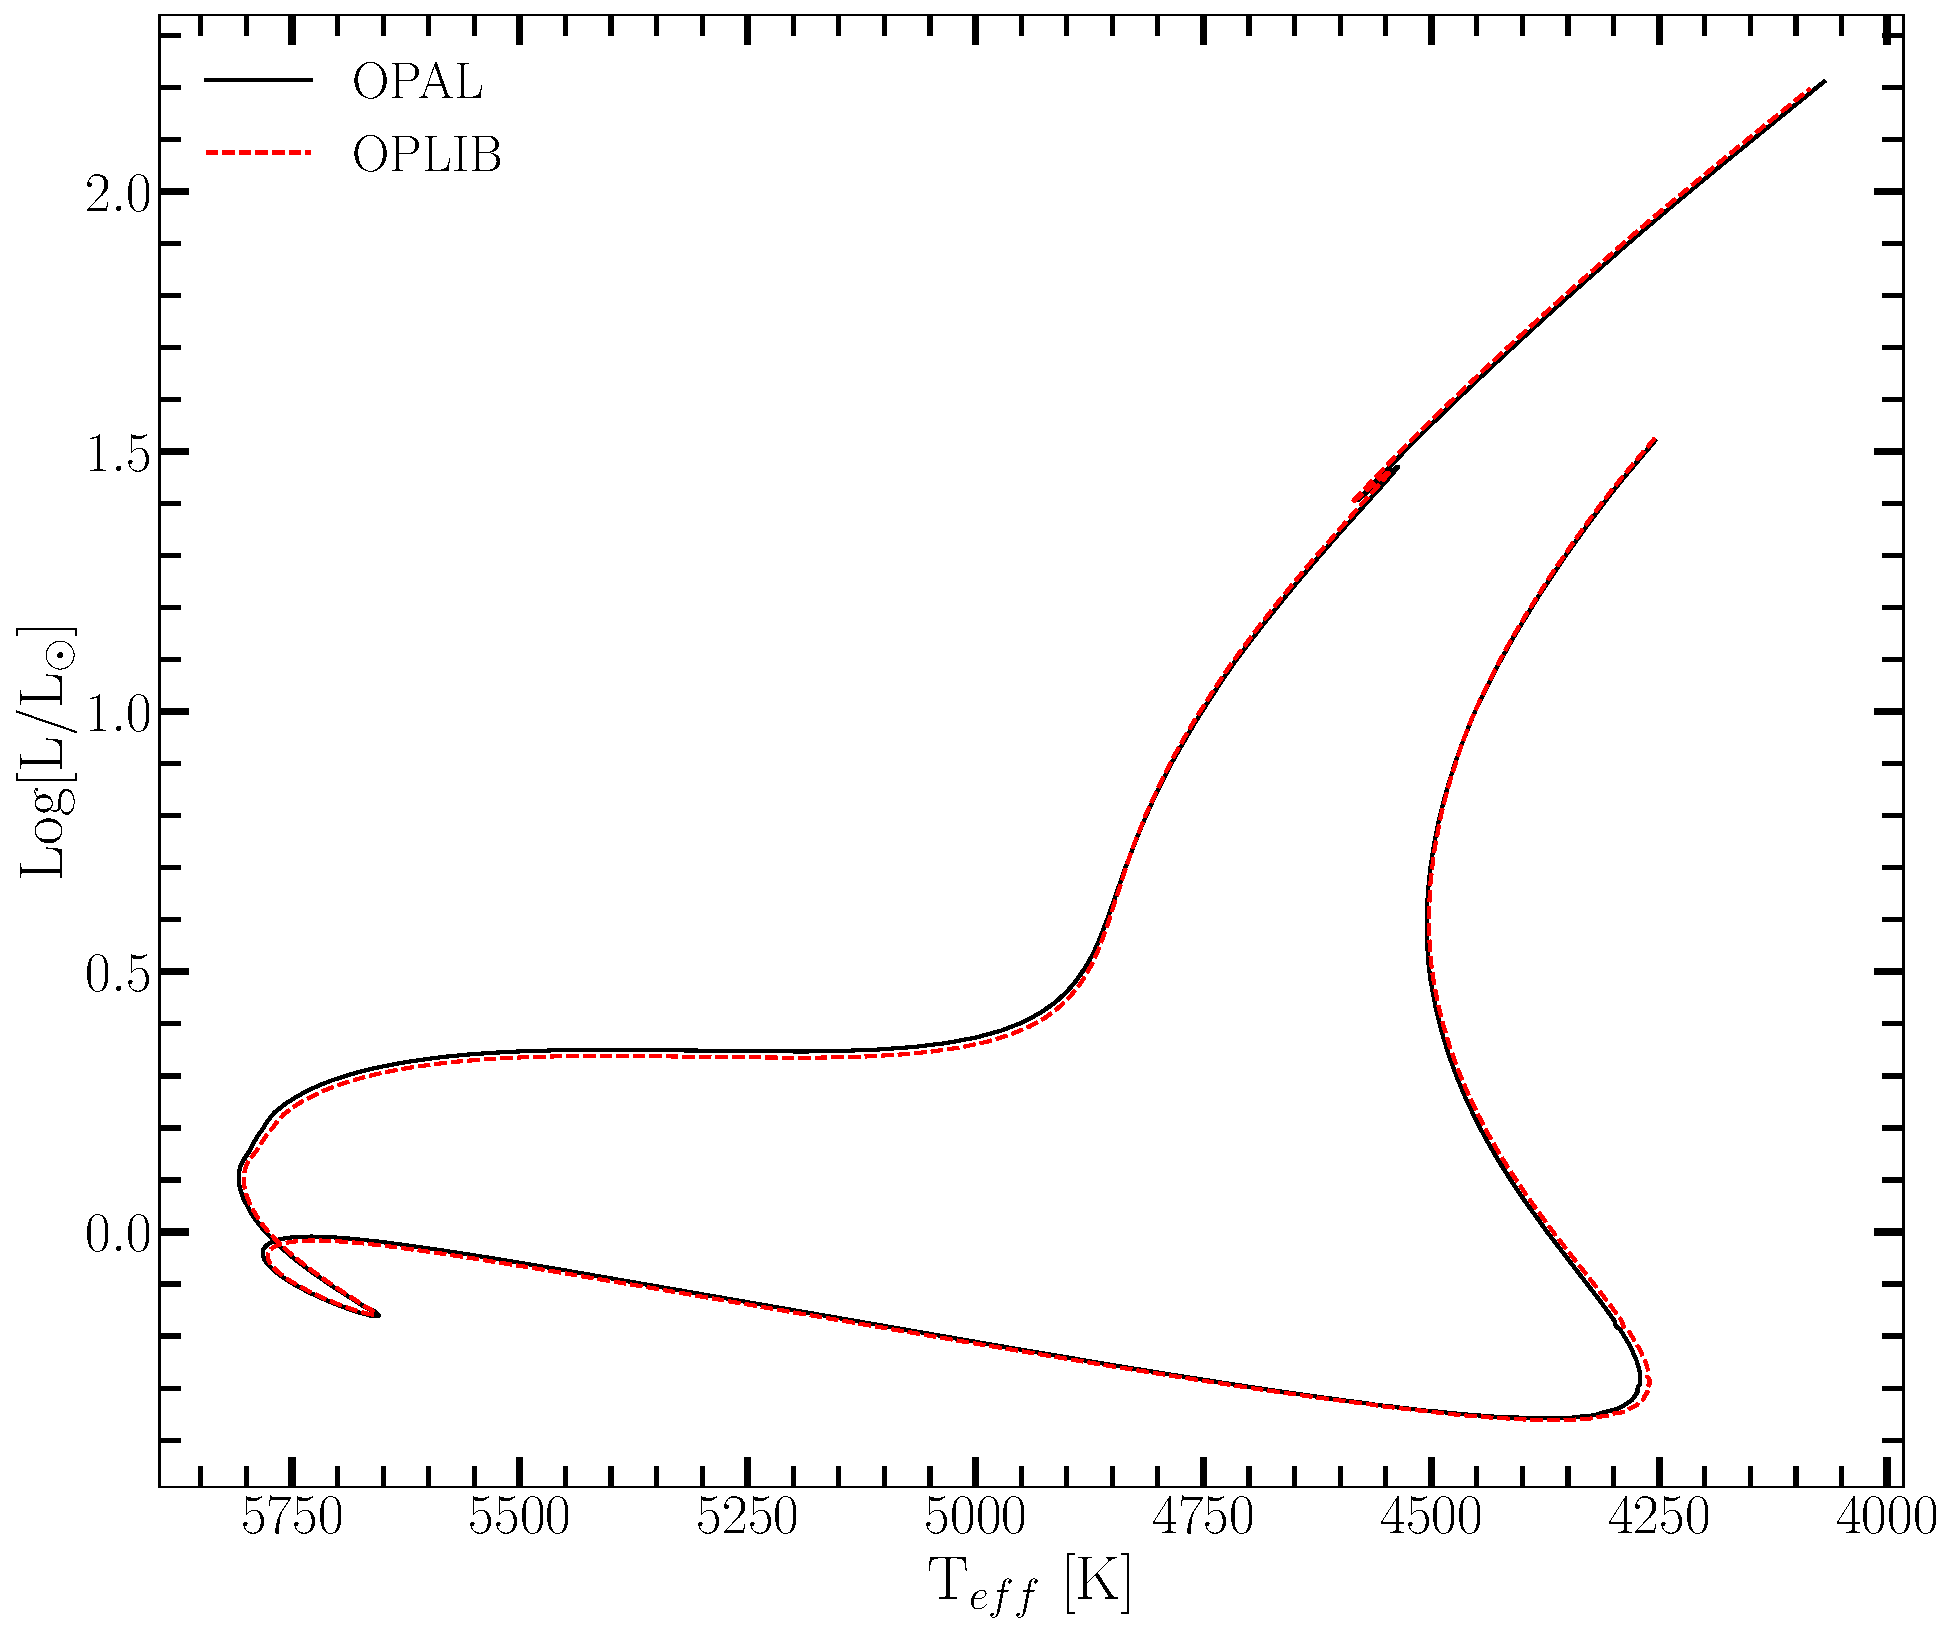
\includegraphics[width=0.20\textwidth]{src/Figures/HRDiagramOPALvsOPLIB_SCCM.pdf}
			\end{tikzfigure}

			For $\log(R)=-1.5$, OPAL and OPLIB opacities vary up to
			approximately 2\% when $T\geq10^{6}$ K. The calibrated solar model
			above shows that variations of this order are not expected to
			dramatically alter a stars evolutionary path. However, these small
			variations may be more impactful for stars at or near the
			convective transition mass where small changes in $\kappa$ can
			result in large changes in $T$ for a constant $\nabla_{rad}$.
	    }
	
		\block{Modeling}{
			
		}

	    \block{Acknowledgments}{
				This research has made use of NASA's astrophysical data system
				(ADS). We acknowledge the support of an NASA grant (No.
				80NSSC18K0634). Additionally, we would like to thank James
				Colgan for his assistance with the OPLIB opacity tables. We
				would like to thank Aaron Dotter, and Elisabeth Newton for
				their assistance. Finally, we thank our colleagues and peers in
				for their continuing and appreciated support.


            }

	    \column{0.66}
		\block{Modeling the Gap}{
			A theoretical explanation for the Jao Gap comes from
			[CITE], who propose that in a star directly above the
			transition mass, due to asymmetric production and destruction of
			He$^{3}$ during the proton-proton I chain (ppI), periodic
			luminosity variations can be induced. This process is known as
			convective-kissing instability. Such a star will descend the pre-MS
			with a radiative core; however, as the star reaches the zero age
			main sequence (ZAMS) and as the core temperature exceeds $7\times
			10^{6}$ K, enough energy will be produced by the ppI chain that the
			core becomes convective. At this point the star exists with both a
			convective core and envelope, in addition to a thin, radiative,
			layer separating the two. Subsequently, asymmetries in ppI affect
			the evolution of the star's convective core.
			
	        \begin{tikzfigure}[Internal Evolution of a star experiencing convective kissing instabilities.]
	        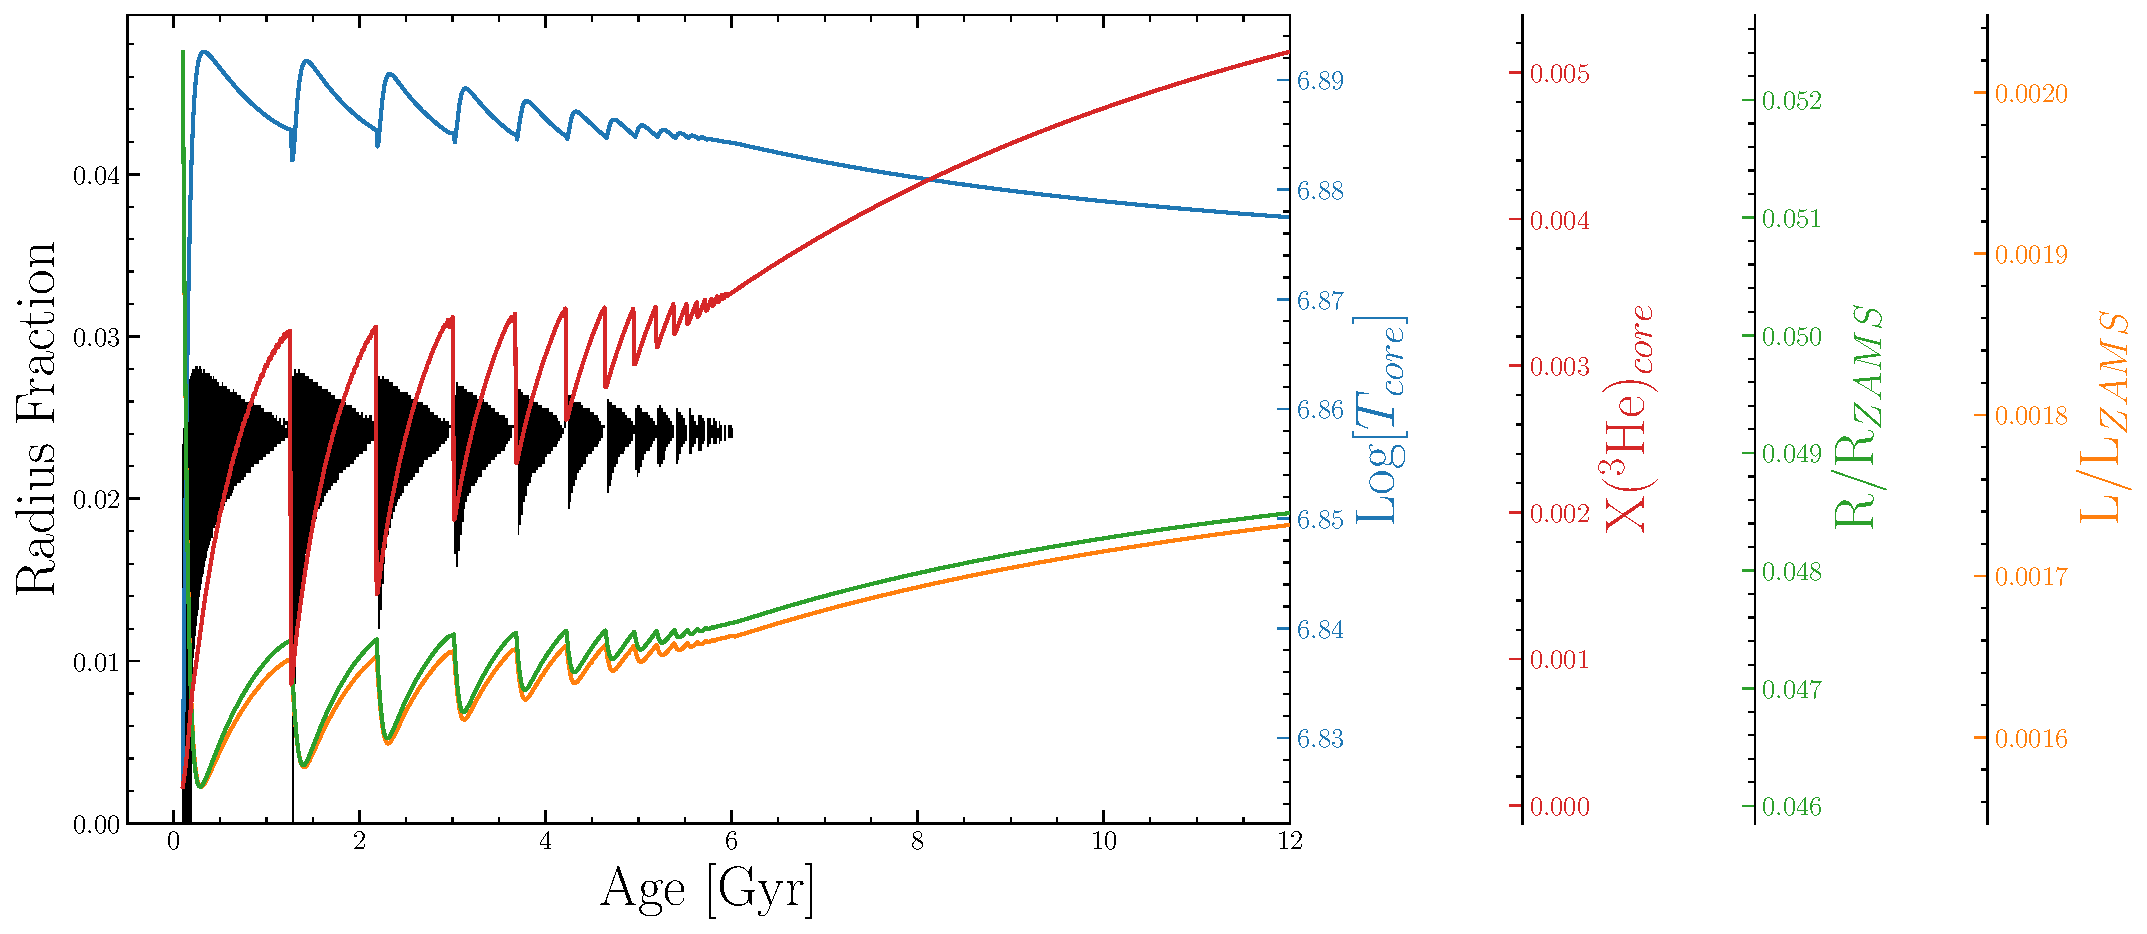
\includegraphics[scale=1]{src/Figures/Kippenhan.pdf}
	        \end{tikzfigure}

			We evolve a set of models with very finely spaced masses (between
			0.2 and 0.8 M$_{\odot}$, dM=0.002 M$_{\odot}$) using the Dartmouth
			Stellar Evolution Program (DSEP, Dotter et al. 2008)

	        \begin{tikzfigure}[Jao Gap in population synthetis]
	        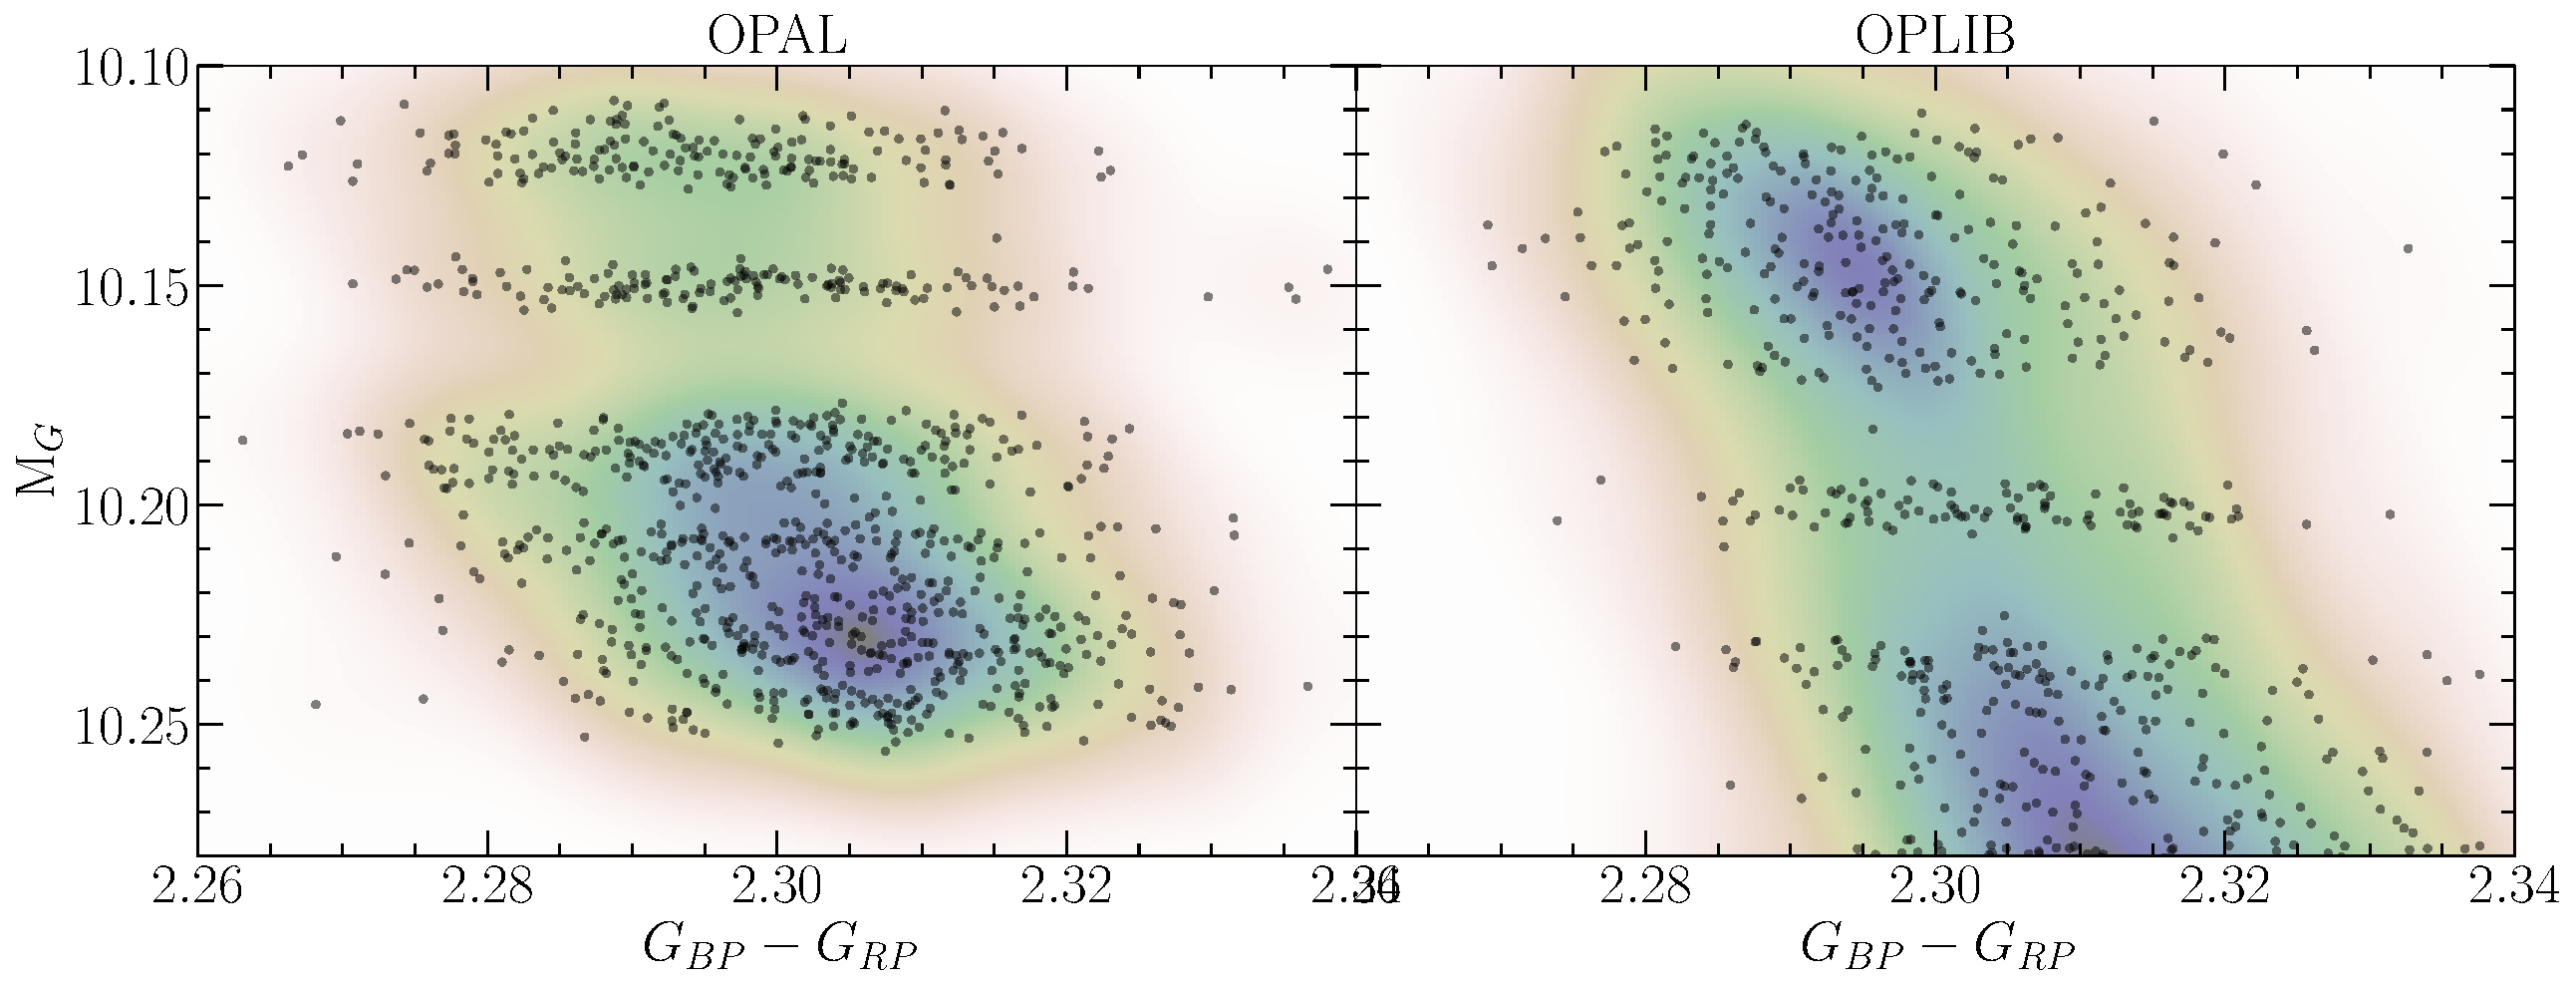
\includegraphics[scale=1]{src/Figures/OPALOPLIB_popsynth_comp.pdf}
	        \end{tikzfigure}

	    }

		% \column{0.25}
        %
		% \block{Population Synthethis}{
		% 	We 
        %
		% }
        %
	    % \block{{Acknowledgments}}{
	    %     {\fontsize{20}{25}\selectfont
		% 		This research has made use of NASA's astrophysical data system
		% 		(ADS). We acknowledge the support of an NASA grant (No.
		% 		80NSSC18K0634). Additionally, we would like to thank James
		% 		Colgan for his assistance with the OPLIB opacity tables. We
		% 		would like to thank Aaron Dotter, and Elisabeth Newton for
		% 		their assistance. Finally, we thank our colleagues and peers in
		% 		for their continuing and appreciated support.
        %         
        %         
        %     \vspace{-2cm}
        %     }}
        % \block{References}{
        % {\fontsize{20}{25}\selectfont
        %     \begin{enumerate}
        %         \item U. Heber. Hot Subluminous Stars. Publications of the Astronomical Society of the Pacific, 128(8):082001, August 2016. 10.1088/1538-3873/128/966/082001.
        %      \end{enumerate}
        %  }
        % }
	\end{columns}
\end{document}
